%%%%%%%%%%%%%%%%%%%%%%%%%%%%%%%%%%%%%%%%%%%%%%%%%%%%%%%%%%%%%%%%%%%%
\section{Overview}
\label{sec:fd-daq-ov}

\metainfo{DP/SP shared.  Georgia Karagiorgi and Dave Newbold. 2 Pages - largely
  generic but some highlighting of SP-specifics. 
  Focus on describing to HEP but non-DAQ expert. 
  Include how design is resilient in the face of potential
  uncertainties such as excess noise or the need to reduce drift HV
  (just two examples, maybe there are more).}

%%%%%%%%%%%%%%%%%%%%%%%%%%%%%%%%%
\subsection{Introduction}
\label{sec:fd-daq-intro}

The DUNE \dword{fd} \dword{daq} system must enable the readout,
triggering, processing and distribution to permanent storage of data
from all \dwords{detmodule} which includes both their electrical
\dword{tpc} and optical \dword{pds} signals.  
The final output data must retain, with very high efficiency and low
bias, a record of all activity in the detector which pertains to the
recognized Physics goal of the DUNE experiment. 
The practical constraints of managing this output requires that the
DAQ achieve these goals while reducing the input data by almost four
orders of magnitude.

The current generation of LArTPC DAQ, such as used in
\dword{protodune} and \microboone, record data over a fixed window of
time which is chosen based on the acceptance of an external trigger. 
The DUNE DAQ faces several major challenges beyond those of the
current generation. 
Foremost, it must accept data from an order of magnitude more channels
and from that data it must form its own triggers.
This self-triggering functionality requires immediate processing of
the full-stream data from a large portion of all TPC channels with a
throughput of approximately one terabyte per second per
\dword{detmodule}. 
The nature of various technical, financial and physical constraints
leads to much of the computing hardware to host this processing to
reside underground and near to the detector modules.

Past LArTPC and long-baseline neutrino detectors have successfully
demonstrated external triggering using information related to their
associated particle beam. 
And indeed the DUNE FD DAQ will accept external information on recent
times of Main Injector beam spills from Fermilab. 
This will assure triggering with high efficiency to capture activity
pertaining to interactions from the produced neutrinos. 

However, even if the DUNE experiment had no physics goals other than
those related to neutrinos from these beam spills, an external beam
trigger alone is not sufficient. 
Absent any other information, such a trigger must inevitably call for
the readout of all possible data from the FD over a period of time of
at least as one LArTPC drift time. 
This would lead to an annual data volume approaching an exabyte
($10^{18}$ bytes) the vast majority of which consists of just noise. 
This entire data volume would have to be saved to permanent storage
and then processed offline in order to get to the signals.

Of course, DUNE does have a broad set of physics goals which expands
to include also the observation of interactions and decays that are
unrelated to the beam of neutrinos from Fermilab. 
This activity includes cosmic ray muons, which provide an important
source of detector calibration, and atmospheric neutrino interactions,
that give a secondary source from which to measure neutrino
properties. 
Taken together, and detailed below, recording their activity will
dominate the data rate.
The DAQ must also record data with sensitivity to rare interactions
(both known and hypothetical) such as nucleon decay, other baryon
number violating processes (such as neutron-antineutron oscillation),
and interactions from the products of \dwords{snb}. 

Some of these events, while rare in themselves, produce patterns of
activity that can be mimicked by other higher rate backgrounds.
In the case of supernova neutrino bursts this is particularly so. 
While the exact processes involved in SNBs are not fully understood,
it is expected that a prolonged period of activity of many tens of
seconds will occur over which their neutrino interactions may be
observed. 
Individually, these interactions will be of low energy (relative to
that of beam neutrino interactions, for example) and will be spread
over time and the bulk of the \dwords{detmodule}. 
Because of their signature and their importance, special attention is
required to first ascertain that a SNB may be occurring and to save as
much data as possible over their duration.

Thus the DAQ must greatly reduce the full-stream of its input data
while using the data itself to do so. 
It must do this efficiently both in terms of recording essentially all
activity important to the physics goals of DUNE and in terms of
output data at a rate which is manageable.  


\subsection{Design Considerations}
\label{sec:fd-daq-des-consid}

The different \dwords{detmodule} have variation in terms of their
readout technology and schemes, timing system, channel counts and data
throughput and format.
All of this determines the nature of the digital data which is input
to the DAQ. 
The design of the DAQ strives to contain the unique layers which adapt
to the variation in \dwords{detmodule} toward its ``front end'' in
order to allow as many of its ``back end'' components identical across
the \dwords{detmodule} as possible. 
In particular, the DAQ presents a unified interface to the ultimate
consumer of its data, the DUNE offline computing.
It must also accept and process the data from a variety of other
sources including the accelerator, various calibration systems
(including laser, cold electronics, photodetectors, and potentially
others) as well as trigger sources external to DUNE. 
The daq must be optimized for the above while also retaining
flexibility to scale to handle certain risks such as excess noise,
changes in high voltage, cut network connectivity and other credible
potentialities.

\begin{dunefigure}[DAQ Overview]{fig:daq-overview}
  {The high-level design for the DUNE FD DAQ showing data (solid, with
    line width indicating throughput) and trigger (dashed) flows. 
    A detector module has specialized implementation of some of these
    high level components, particularly toward the upstream front-end
    as described in the text. 
    The grayed boxes are not in the DAQ scope.
    See text for details.
}
% This PDF is made from the .dot of the same name.
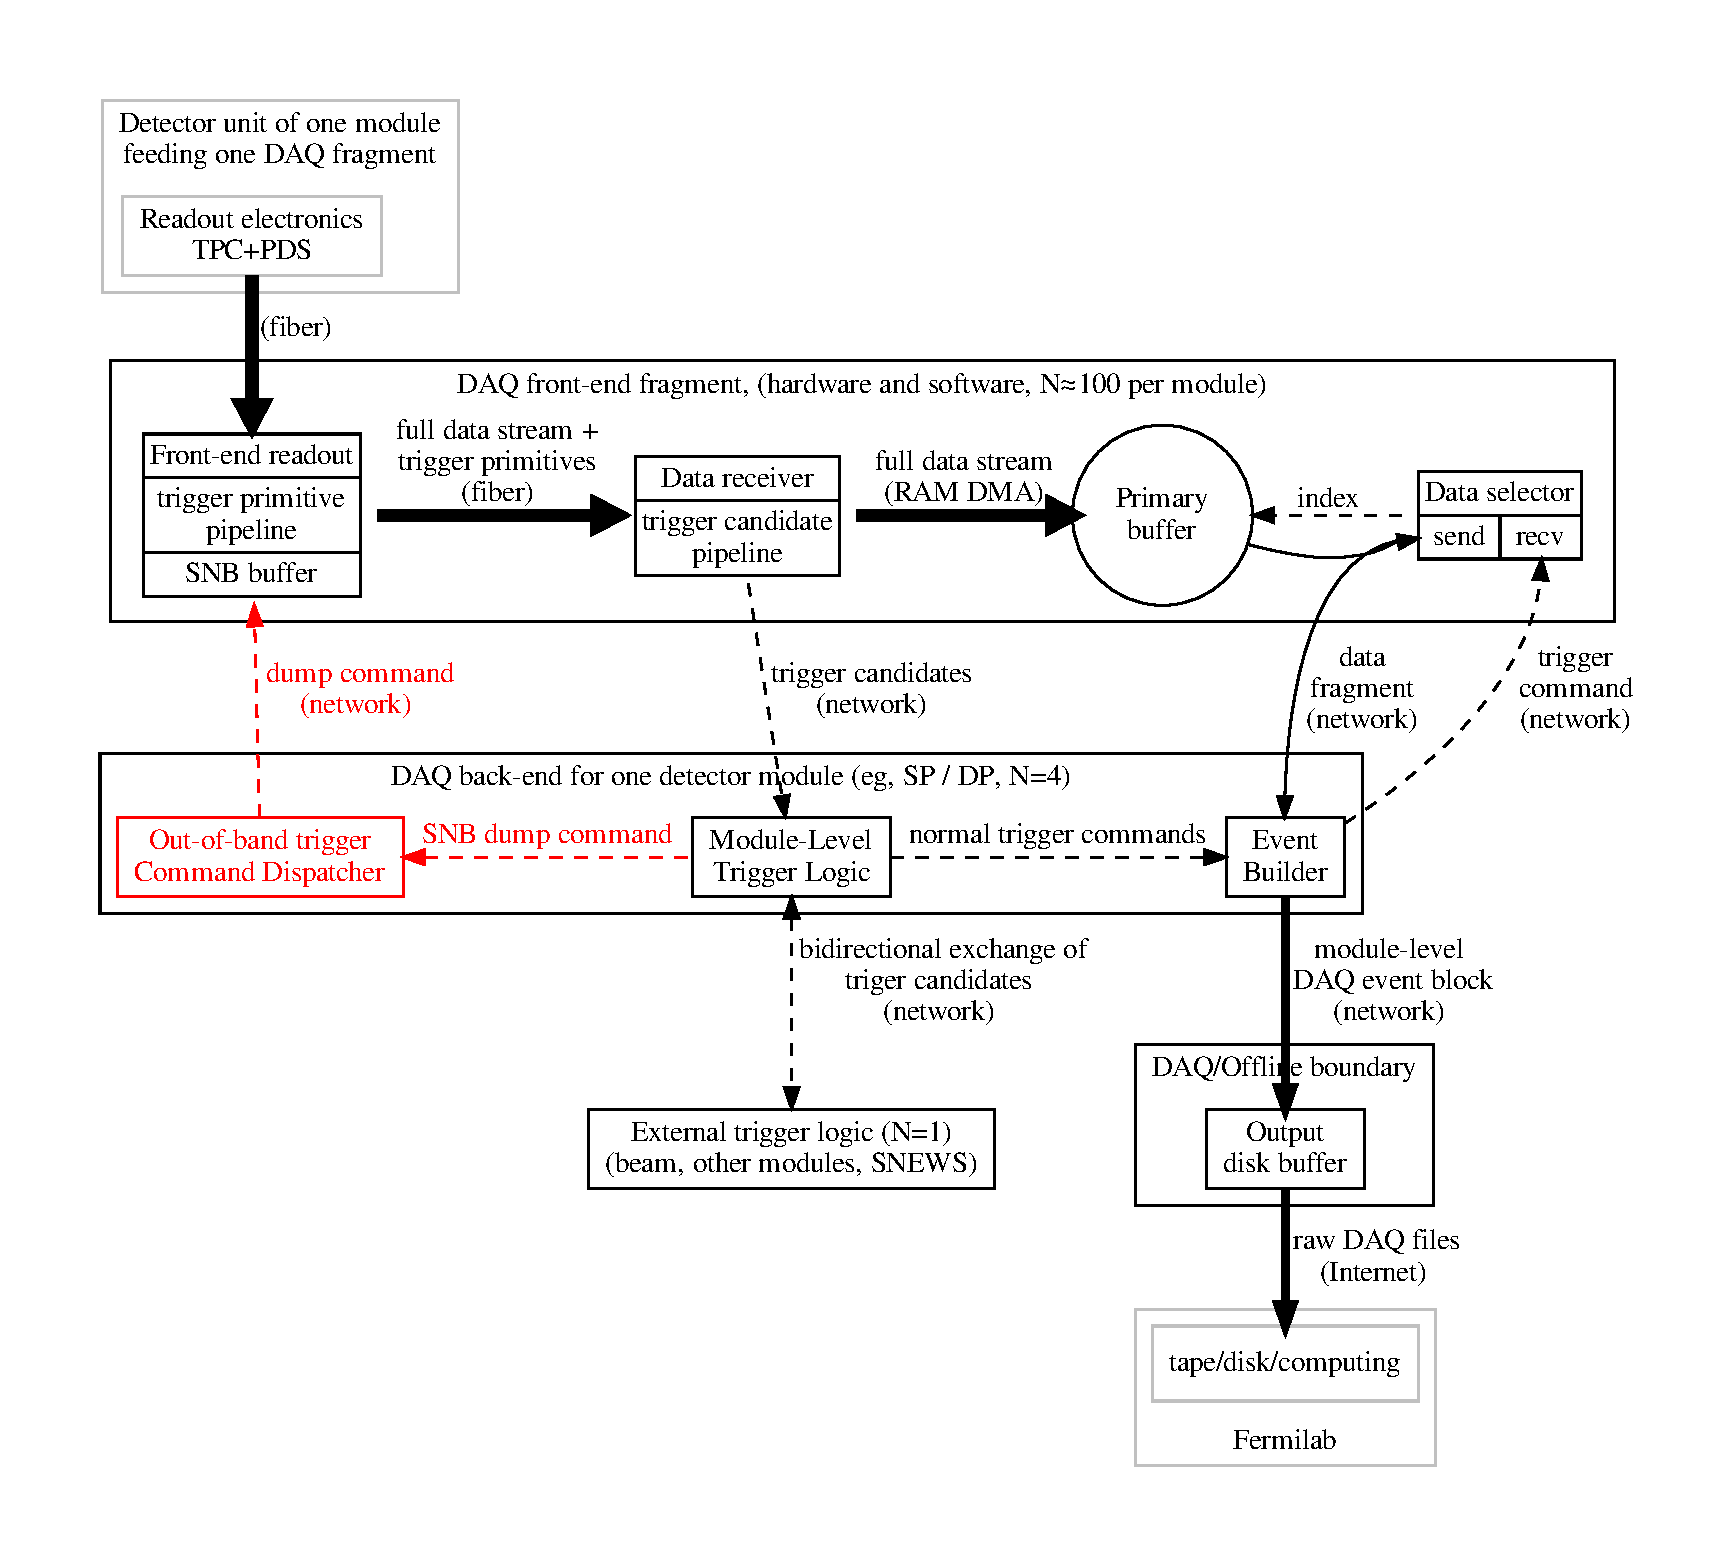
\includegraphics[width=0.8\textwidth]{high-level-daq.pdf}%
\end{dunefigure}


Figure~\ref{fig:daq-overview} gives an illustration of the high-level
DUNE FD DAQ design in terms of data and trigger flow.
At this level of detail the diagram is generic to all
\dwords{detmodule} but some of the depicted roles will necessarily
have implementation specific to their \dword{detmodule}.
The subsections of Section~\ref{sec:fd-daq-design} give more
description of this high-level design as well as details on
specialized implementations.

The high level requirements for the DUNE FD DAQ are provided in
\cite{daq:reqs}.
The most critical requirements in consideration for the overall design
are summarized in Table~\ref{tab:daqrequirements}.

\begin{dunetable}[Important requirements on the DAQ system design]
{p{0.2\textwidth}p{0.6\textwidth}}
{tab:daqrequirements}
{Important requirements on the DAQ system design}   
Requirement  & Description \\ \toprowrule
Scalability & The DUNE FD DAQ shall be capable of receiving and
buffering the full raw data from all four FD modules \\ \colhline 
Zero deadtime & The DUNE FD DAQ shall operate without deadtime under
"normal" operating conditions \\ \colhline
Triggering & The DUNE FD DAQ shall provide full-detector triggering
functionality as well as self-triggering
functionality; the data selection shall maintain high efficiency to
physics events while operating within a total bandwidth of 30 PB/year
for all operating FD modules \\ \colhline
Synchronization & The DUNE FD DAQ will provide synchronization of
different FD modules to within 1~$\mu$s, and of different subsystems
within a module to within 10~ns\\ \colhline
\end{dunetable}

The input bandwidth and processing needs of the DAQ are expected to be
dominated by the rate of data produced by the TPC system of each
\dword{detmodule}.
These rates vary between the modules and their estimations are summarized in
Table.~\ref{tab:daq-input-bandwidth}.
\begin{dunetable} [Pre-trigger data rates from the DUNE FD TPCs and into DAQ front end.]
  {lll} {tab:daq-input-bandwidth} {The parameters governing the pre-trigger data rate from units of each \dword{detmodule} TPC \dwords{ce} and the aggregate throughput into the \dwords{fec} of the DAQ \dwords{daqfrag}.  Compression is an estimate and will be reduced if excess noise is introduced.  
  }
  parameter & \dlong{sp} & \dlong{dp} \\
  \colhline
  TPC unit & APA & CRO crate \\
  unit multiplicity & 150 & 240 \\
  channels per unit & 2560 (800 collection) & 640 (all collection) \\
  ADC sampling & \SI{2}{\MHz} & \SI{2.5}{\MHz} \\
  ADC resolution & 12 bit & 12 bit \\
  \colhline
  aggregate from \dword{ce} & \SI{1440}{\GB/\s} & \SI{576}{\GB/\s} \\
  compression factor & 5$\times$ (in \dshort{daqfer}) & 10$\times$ (in \dshort{cro} crate) \\
  aggregate to FEC & \SI{230}{\GB/\s} & \SI{58}{\GB/\s} \\
  \colhline
\end{dunetable}

The ultimate limit on the output data rate of the DUNE FD DAQ is
expected to be provided by the available bandwidth to and the tape,
disk and processing capacity of Fermilab. 
An ample guideline has been established which places this limit at
about \offsitepbpy or \offsitegbps.
Extrapolating to four FD detector modules this requires the DAQ to
perform a data reduction factor of almost four orders of magnitude. 
This will be achieved through a simple self-triggered readout strategy.

An overestimate of the annual, triggered data volume assuming the FD
is comprised of four \dword{sp} \dwords{detmodule} is summarized in
Table.~\ref{tab:daq-data-rates}. 
It assumes a very generous and simple trigger scheme whereby the data
from the entire \dword{detmodule} is saved for a period longer than
two drift times around the trigger time.
This essentially removes selection bias at the cost of producing
substantially more data.
It is important to note that as generous as this scheme is, the
overestimate meets the required data reduction factor described above.  
It is expected that future studies, including early data taking, will
discover ways to reduce the data volume while retaining high selection
efficiency and low bias.

\begin{dunetable}
[Anticipated event and data rates assuming four SP modules.]
{p{0.25\textwidth}p{0.15\textwidth}p{0.4\textwidth}}
{tab:daq-data-rates}
{Anticipated event and data rates assuming four SP modules. The
  rates assume continuous readout (without any data reduction) for
  5.4~ms for non-extended events, and for 10 seconds for extended events.}   
Event Type  & Annual Data Volume & Assumptions \\ \toprowrule
 Beam interactions & 27 TB & 800 beam and 800 dirt muons; 10~MeV
 threshold in coincidence with beam time; include cosmics\\ \colhline
 Cosmics and atmospherics & 10 PB &  \\ \colhline
 Radiologicals & $\le$1~PB & fake rate of $\le$100 per year \cite{daq:simreport}\\ \colhline
 Front-end calibration & 200~TB & Four calibration runs per year, 100
 measurements per point \\ \colhline
 Radioactive source calibration & 100~TB & source rate $\le$10~Hz;
 single APA readout; lossless readout \\ \colhline
 Laser calibration & 200~TB & 1$\times$10$^6$ total laser
 pulses, lossy readout \\ \colhline
 Random triggers & 60 TB & 45 per day\\ \colhline
 Trigger primitives & $\le$6~PB &  all three wire planes; 12 bits per
 primitive word; 4 primitive quantities; $^{39}$Ar-dominated\\ \colhline
\end{dunetable}


It assumes the level of noise is consistent with the expected,
intrinsic, thermal noise of the electronics.
Trigger rates increase and compression factors decrease in a manner
that is sensitive to the amount and type of excess noise, such as can
be due to \dword{rf} emission inside the cryostat. 
Future studies may be done over a variety of guesses for different
possible excess noise scenarios and they will receive beneficial input
from the results of \dword{protodune}.

\fixme{Table~\ref{tab:daq-data-rates} is really unclear.  Need to clarify the physical origin, trigger and readout type for each one. Assumptions also include quite a bit of jargon.}

\fixme{Table~\ref{tab:daq-data-rates} - 10s for extended events is out of date. What are we saying ?}

\fixme{Table~\ref{tab:daq-data-rates} does not include 5x compression, right?  If not, it should be adjusted to include it.}

\fixme{Table~\ref{tab:daq-data-rates} should add SNB data.}

\fixme{Table~\ref{tab:daq-data-rates}, caption and text should maybe divide by 4 and say it's just SP.  We can have a summary statement where we extrapolate to SP+DP+M3+M4.}




%%%%%%%%%%%%%%%%%%%%%%%%%%%%%%%%
\subsection{Scope}
\label{sec:fd-daq-scope}

%\metainfo{This section may also wish to refer to Fig.~\ref{fig:daq-overview}.}

The nominal scope of the \dword{daq} system is illustrated in
Fig.~\ref{fig:daq-overview} by the boxes which are not grayed out and
includes the continued procurement of materials for, and the
fabrication, testing, delivery and installation of the following
systems:

\begin{itemize}
\item Front-end readout hardware and firmware/software development for \dword{trigprimitive} generation.
\item Front-end computing for hosting of \dword{daqdr}, \dword{ringbuffer} and \dword{daqds}.
\item Back-end computing for hosting \dword{mtl}, \dword{eb} and the \dword{daqoob} processes.
\item External trigger logic and its host computing.
\item Algorithms to generate trigger commands which perform data selection.
\item Timing distribution system
\item DAQ data handling software including receiving and building of
  events
\item Run control software, configuration database, and user interface
\item Rack infrastructure in the central utility cavern for readout
  electronics, front-end computing, timing distribution, and data
  selection
\item Rack infrastructure on surface at SURF for back-end computing
\end{itemize}


